\chapter{Quasi-Deterministic and Event-Driven Programming with LVars\label{ch:quasi}} % 2

\TODO{Move Listings junk out of here.}

\newcommand{\figbfs}{
\begin{table}[H]
\begin{center}
\begin{tabular}{c | c | c | c | c | c | c}
         & verts & seq  & best    & best  & work/ & verts/  \\ 
         & $\times 10^6$    & time & speedup & cores & vert  & sec   \\ \hline 
 BFS IStruct         & 0  & 0 & 0  & 0  & 0 & 0 \\ \hline 
 BFS IStrct/unbox    & 0  & 0 & 0  & 0  & 0 & 0 \\ \hline 
 BFS linked Set      & 0  & 0 & 0  & 0  & 0 & 0 \\ \hline 
 BFS no work         & 0  & 0 & 0  & 0  & 0 & 0 \\ \hline 
\hline 
 MIS IStruct         & 0  & 0 & 0  & 0  & 0 & 0 \\ \hline 
 MIS IStrct/unbox    & 0  & 0 & 0  & 0  & 0 & 0 \\ \hline 
 MIS linked Set      & 0  & 0 & 0  & 0  & 0 & 0 \\ \hline 
 MIS no work         & 0  & 0 & 0  & 0  & 0 & 0 \\ \hline 
\end{tabular}
\end{center}
\caption{Throughput in vertices per second as a function of per-vertex task size.}
\label{fig:bfs}
\end{table}
}

Programs written using a \emph{deterministic-by-construction} model of
parallel computation are guaranteed to always produce the same
observable results, offering programmers freedom from subtle,
hard-to-reproduce nondeterministic bugs.  While a number of popular
languages and language extensions (\eg, Cilk~\cite{cilk}\lk{Any
  others?}) \emph{encourage} deterministic parallel programming, few
of them guarantee determinism for \emph{all} programs written using
the model.

Of the options available to programmers for
deterministic-by-construction parallel programming, perhaps the most
mature and broadly available choice is pure functional programming
with function-level task parallelism, or \emph{futures}.  For example,
Haskell programs using futures by means of the @par@ and @pseq@
combinators can provide real speedups on practical programs while
guaranteeing determinism~\cite{marlow-par}.\footnote{The determinism
  guarantee only obtains if user programs are written in the
  \emph{Safe Haskell}~\cite{safe-haskell} subset of Haskell (which is
  implemented in GHC Haskell by means of the \lstinline|SafeHaskell|
  language pragma), and if they do not use the \lstinline|IO| monad.}
Yet pure programming with futures is not ideal for all problems.
Consider a \emph{producer/consumer} computation in which producers and
consumers can be scheduled onto separate processors, each able to keep
their working sets in cache.  Such a scenario enables \emph{pipeline
  parallelism} and is common, for instance, in stream processing.  But
a clear separation of producers and consumers is difficult with
futures, because whenever a consumer forces a future, if it is not yet
available, the consumer immediately switches roles to begin computing
the value (as explored by Marlow \etal~\cite{monad-par}).

Since pure programming with futures is a poor fit for
producer/consumer computations\lk{are we brave enough to say ``a poor
  fit''?  there's also ``less than ideal''}, one might then turn to
{\em stateful} deterministic parallel models.  Shared state between
computations allows the possibility for race condition that introduce
nondeterminism, so any parallel programming model that hopes to
preserve determinism must do something to tame sharing---that is, to
restrict access to mutable state shared among concurrent computations.
Systems such as DPJ (Deterministic Parallel Java)~\cite{dpj-hotpar09}
and Concurrent
Revisions~\cite{concurrent-revisions-oopsla,concurrent-revisions-haskell11},
for instance, accomplish this by ensuring that the state accessed by
concurrent threads is {\em disjoint}.

We are concerned with an alternative approach: allowing {\em data} to
be shared, but limiting the {\em operations} that can be performed on
it to only those operations that commute with one another and thus can
tolerate nondeterministic thread interleavings.  Although the order in
which side-effecting operations occur can differ on multiple runs, a
program will always produce the same externally observable
result.\footnote{There are many ways to define what is observable
  about a program. We define the observable result of a program to be
  the value to which it evaluates.\lk{Maybe I should explain this
    further?  Or point back to where I discussed it in
    Chapter~\ref{ch:intro}?}}  Specifically, we are concerned with
models where shared data structures grow {\em monotonically}---by
publishing information, but never invalidating it.  Consider two
classic deterministic parallel models, dating back to the late 60s and
early 70s\lk{Is it a problem that some of the following text is reused
  from Chapter~\ref{ch:intro}?}:
\begin{itemize}
\item In {\em Kahn process networks} (KPNs)~\cite{Kahn-1974}, as well
  as in the more restricted {\em synchronous data flow}
  systems~\cite{Lee-sdn}, a network of processes communicate with each
  other through blocking FIFO channels.  KPNs are the basis for
  deterministic stream-processing languages such as
  StreamIt~\cite{streamit-asplos}, which are narrowly focused but have
  shown clear benefits in auto-parallelization and hardware
  portability.
\item In parallel {\em single-assignment
  languages}~\cite{Tesler-1968}, ``full/empty'' bits are associated
  with heap locations so that they may be written to at most once.
  Single-assignment locations with blocking read semantics are known
  as \emph{IVars}~\cite{IStructures} and are a well-established
  mechanism for enforcing determinism in parallel settings: they have
  appeared in Concurrent ML as @SyncVar@s~\cite{reppy-cml-book}; in
  the Intel Concurrent Collections (CnC) system~\cite{CnC}; in
  languages and libraries for high-performance computing, such as
  Chapel~\cite{chapel} and the Qthreads library~\cite{qthreads}; and
  have even been implemented in hardware in Cray MTA
  machines~\cite{cray-mta}.  Although most of these uses incorporate
  IVars into already-nondeterministic programming environments, the
  \emph{monad-par} Haskell library~\cite{monad-par} uses IVars in a
  deterministic-by-construction setting, allowing user-created threads
  to communicate through IVars without requiring the @IO@ monad.
  Rather, operations that read and write IVars must run inside a @Par@
  monad, thus encapsulating them inside otherwise pure programs, and
  hence a program in which the only effects are @Par@ effects is
  guaranteed to be deterministic.
\end{itemize}

\noindent In KPNs and other data-flow models, communication takes
place over blocking FIFO queues with ever-increasing \emph{channel
  histories}, while in IVar-based programming models such as CnC and
monad-par, a shared data store of blocking single-assignment memory
locations grows monotonically.  Hence \emph{monotonic data
  structures}---data structures to which information can only be added
and never removed---emerge as a common theme of both data-flow and
single-assignment models.

Because state modifications that only add information and never
destroy it can be structured to commute with one another and thereby
avoid race conditions, it stands to reason that diverse deterministic
parallel programming models would leverage the principle of
monotonicity.  Yet systems like CnC, monad-par, and StreamIt emerge
independently, without recognition of their common basis.  Moreover,
because they are based on a single data structure, these programming
models lack \emph{generality}: IVars and FIFO streams alone cannot
support all producer/consumer applications, as we discuss in
Section~\ref{s:lvars-motivation}.

By taking monotonicity as a starting point, then, we can provide a new
model for deterministic parallelism that generalizes existing models
and can guide the design of new ones.  Our model generalizes IVars to
\emph{LVars}, thus named because the states an LVar can take on are
elements of an application-specific {\em lattice}.\footnote{ As we
  will see in Section~\ref{s:lvars-domains}, this ``lattice'' need
  only be a {\em bounded join-semilattice} augmented with a greatest
  element $\top$, in which every two elements have a least upper bound
  but not necessarily a greatest lower bound.  For brevity, we use the
  term ``lattice'' in place of ``bounded join-semilattice with a
  designated greatest element''.}

In this chapter, I define LVars and use them to define $\lambdaLVar$,
a deterministic parallel calculus with shared state, based on the
call-by-value $\lambda$-calculus.  The $\lambdaLVar$ language is
general enough to subsume existing deterministic parallel languages
because it is parameterized by the choice of lattice.  For example, a
lattice of channel histories with a prefix ordering allows LVars to
represent FIFO channels that implement a Kahn process network, whereas
instantiating $\lambdaLVar$ with a lattice with ``empty'' and ``full''
states (where $\mathit{empty} < \mathit{full}$) results in a parallel
single-assignment language.  Different instantiations of the lattice
result in a family of deterministic parallel languages.

As the main technical result of this chapter, I give a proof of
determinism for $\lambdaLVar$ (Section~\ref{section:proof}).  A
critical aspect of the proof is a ``frame'' property, expressed by the
Independence lemma (Section~\ref{s:lvars-independence}), that would
{\em not} hold in a typical language with shared mutable state, but
holds in our setting because of the monotonic semantics of LVars.

Because lattices are composable, any number of diverse monotonic data
structures can be used together safely.  Moreover, as long as we can
demonstrate that a data structure presents the LVar interface, it is
fine to use an existing, optimized concurrent data structure
implementation; we need not rewrite the world's data structures to
leverage the $\lambdaLVar$ determinism result. I discuss how to
formulate a few common data structures (pairs, arrays, FIFOs) as
lattices (Sections~\ref{s:lvars-domains} and
\ref{s:lvars-programming-with-put-and-get}) and how to implement
operations on them within the $\lambdaLVar$ model.

The material in this chapter is based on research done jointly with
Ryan Newton~\cite{LVars-paper, LVars-tr}.

\lk{Mostly edited up to this point.}


%====================================================================================================
%\section{Motivation: Example Application}\label{section:motivation}
\section{Motivating Example: A Parallel, Pipelined Graph Computation}\label{section:motivation}

%% Programming models enabling sharing of a single data structure 
%% necessarily have limited applicability, which is perhaps why even the stream
%% processing languages have not been widely adopted.
%% %% \lk{I think ``programming models built on a single data structure'' is
%% %%   a straw man and the mention of stream languages is a distraction.
%% %%   Saying that, for instance, KPNs are ``built on a single data
%% %%   structure'' because they use FIFOs for communication seems like too
%% %%   much.  I think we can make the case that graph algorithms are a
%% %%   challenge for deterministic parallel languages, without having to go
%% %%   to that length.}
%% % \rn{Now it more specifically refers to SHARING through a single data structure.}
%% %

What applications motivate going beyond IVars and FIFO streams?
% We argue that any application domain is a candidate if it includes
Consider applications in which 
independent subcomputations contribute information to shared data
structures that are {\em unordered, irregular, or application-specific}.
\lk{What does ``application-specific'' mean?}
%{An example application that uses rich, shared data structures and that
%  processes irregular data is}
 Hindley-Milner type inference is one example: in a
  parallel type-inference algorithm, each type variable monotonically
  acquires information through unification (which can be represented as a
  lattice).
%% LK: Not wild about this footnote.  After all, LVars have that
%% problem, too.  Also, it's not *that* tempting ot try to represent
%% type variables as IVars because they don't capture anything about
%% gradually acquiring type informations.
%% \footnote{It is tempting to try to represent type variables as IVars, but
%%   an empty IVar is not a good representation for an
%%   uninstantiated type variable, since checking for emptiness is not allowed.}
 Likewise, in control-flow analysis, the {\em set} of locations to which a variable
 refers monotonically {\em shrinks}.  In logic programming, a parallel
 implementation of conjunction might asynchronously add information to a logic
 variable from different threads.

To illustrate the issues that arise in computations of this nature, we consider a specific problem, drawn from the domain of {\em graph algorithms}, where
 issues of ordering create a tension between parallelism and
determinism:
\begin{itemize}
\item 
  In a directed graph, 
  % Implement a breadth-first-search in a graph to 
  find the connected
  component containing a vertex $v$, and compute a (possibly expensive) function $f$ over 
all vertices in that component, making the set of results available
    asynchronously to other computations.
\end{itemize}
For example, in a directed graph representing user profiles on a social network
and the connections between them, where $v$ represents a particular
profile, we might wish to find all (or the first $k$
degrees of) profiles connected to $v$, then analyze each profile in that set.\lk{this example is kinda creepy, but I can't
  think of one I like better...}
% A level-synchronized breadth-first-search can provide a 

This is a challenge problem for deterministic parallel programming:
existing parallel solutions~\cite{bfs-pbgl} often use a nondeterministic traversal of the
  connected component
  (even though the final connected component is deterministic),
% , and demands rich primitives.
%% We will use a {\em level-synchronized breadth-first-search} to avoid those
%% problems.
and IVars and streams provide no obvious aid.  For example, IVars cannot accumulate
sets of visited nodes, nor can they be used as ``mark bits'' on visited nodes, since 
they can only be written once and not tested for emptiness.
Streams, on the other hand, impose an excessively strict ordering
for computing the unordered {\em set} of vertex labels in a
connected component.
Yet before considering {\em new} mechanisms, we must also ask if a purely functional
program can do the job.


%% {There is a tension between discovering the connected component in
%%   parallel (which can involve data races) and the need for determinism.}
%% Indeed, graph algorithms in general have motivated recent work on 
%% non-deterministic parallel abstractions \cite{kulkarni2007optimistic}.  BFS
%% algorithms in particular often use non-deterministically selected spanning trees
%% in the process of component discovery.
%% \lk{But the problem statement above didn't say anything about BFS.
%%   You could use DFS to find a connected component, too.}
%% %For example, a parallel breadth-first-search (BFS) typically traverses the
%% %connected component via a {\em nondeterministic} spanning tree (even though the
%% %final set of nodes in the connected component is deterministic).  
%% A typical parallel, imperative BFS implementation associates ``mark bits'' with
%% vertices to mark them as visited (asynchronously).  Using IVars as mark-bits does
%% not work because one may not peek at an IVar to check for emptiness: only
%% blocking reads are allowed.
%% %% \lk{I think the argument here is flawed:
%% %%   * First, we say that IVars don't help with our challenge problem
%% %%   because you can't use IVars as mark bits.  But (a) you don't need to
%% %%   use mark bits to do BFS, and (b) you don't need to do BFS to find a
%% %%   connected component.
%% %%   * Second, after complaining that you can't use IVars as mark bits.
%% %%   we don't present an alternative to IVars that DOES let you use mark
%% %%   bits.  Rather, we present a different, purely functional solution --
%% %%   which is fine, but if that's what we're going for then we shouldn't
%% %%   set up ``You can't use mark bits!'' as the problem in the first
%% %%   place.
%% %% }


%------------------------------------------------------------
\paragraph{A purely functional attempt}
%% {A pure functional program (with futures) can sacrifice some potential
%%   parallelism to make component-discovery deterministic, by using a {\em
%%     level-synchronized} BFS.
%% \lk{The previous sentence is a bit confusing.  It makes it sound like
%%   the level-synchronization has something to do with being purely
%%   functional.  Actually, as far as I can tell, level-synchronization
%%   is the done thing for any parallel BFS, purely functional or
%%   otherwise.  For instance:
%%   \url{}.
%%   I'm going to do some digging to find out where the first reference
%%   for level-synchronized parallel BFS is...}
Figure~\ref{f:bfs-pure} gives a Haskell implementation of 
a {\em level-synchronized} breadth-first traversal,
in which nodes at distance one from the starting vertex are
  discovered---and set-unioned into the connected component---before nodes of
  distance two are considered.  Level-synchronization is a popular strategy for
parallel breadth-first graph traversal (see, for instance, the Parallel Boost Graph Library \cite{bfs-pbgl}), although it necessarily sacrifices
some parallelism for determinism: parallel tasks cannot continue discovering
nodes in the component (racing to visit neighbor vertices) before synchronizing
with all other tasks at a given distance from the start.

%
%% \rn{TODO -- FINISH THIS -- I think it actually works to accumulate a list of
%%   futures in a pure, eager programming language.  Ok, the thing that is at least
%% TRICKY and maybe not possible is publishing those asynchronously.}
%
% To see the limitations of these preexisting models:

Unfortunately, the code given in Figure~\ref{f:bfs-pure} does not
quite implement the problem specification given above.
Even though connected-component discovery is
  parallel, members of the output set do not become available to other computations until component discovery is {\em
    finished}, limiting parallelism.  We could manually push the @analyze@
  invocation inside the @bf_traverse@
  function,
  % LK: what is `check` from?
  %(in @check@)
  allowing the @analyze@ computation to start sooner, but then we push
  the same problem to the downstream consumer, unless we are able to perform a
  heroic whole-program fusion.
  %% \lk{Aha!  Now I see where you're going with this and I think this is
  %%   a key point: we're prevented from PIPELINING the work here because
  %%   we have no monotonicity guarantee.  Kahn 1974 makes a point of
  %%   talking about how in KPNs, monotonicity enables both pipelining
  %%   and determinism.  I think this point is getting lost and we need
  %%   to emphasize it!}
%
%% \rn{Note you can create a library that allows you to map over a set of futures
%%   and return a new set of futures.  And you can carry on in that way.  But
%%   consuming even one element from the final set will wait on the whole
%%   collection.}
%
If @bf_traverse@ returned a list, lazy evaluation could
  make it possible to {\em stream} results to consumers
  incrementally.  But with a {\em set} result, such pipelining is not generally possible:
  consuming the results early would create a proof obligation that the
  determinism of the consumer does not depend on the order in which results
  emerge from the producer.\footnote{As intuition for this idea, consider that purely functional set data
    structures, such as Haskell's \lstinline|Data.Set|, are typically represented with
    balanced trees.  Unlike with
    lists, the structure of the tree is not known until all elements are present.  
    %% A special fusion framework for sets might help, but we believe it
    %% would be hard to predict performance and it is not the solution we pursue in
    %% this paper.
    \lk{Commented out the part about fusion because we already mention
      it in the main text.  And even if we had a fusion framework for
      sets, it would only handle sets, not all of the other data
      structures we care about.  I think we sell ourselves short by
      making too much of the fusion idea.}}

A compromise would be for @bf_traverse@ to return a list of level-sets:
  distance one nodes, distance two nodes, and so on.  Thus level-one results could
  be consumed before level-two results are ready.  Still, the problem would remain: within
  each level-set, we cannot launch all instances of @analyze@ and
  asynchronously use those results that finish {\em first}.
%
Furthermore, we still have to contend with the previously-mentioned
difficulty of separating producers and consumers when expressing
producer-consumer computations using pure programming with futures
\cite{monad-par}.
% and it's not clear from previous work if it is efficient either.



\begin{figure}
  \lstinputlisting{chapter2/code/bfs_pure.hs}
  \caption{\footnotesize A purely functional Haskell program that maps the \lstinline|analyze| function over the connected
    component of the \lstinline|profiles| graph that is reachable from the node \lstinline|profile0|.  Although component discovery proceeds in parallel, results of
    \lstinline|analyze| are not asynchronously available to other computations, inhibiting pipelining.}
  \label{f:bfs-pure}
\end{figure}


%--------------------------------------------------------------------------------
\paragraph{Our solution}
%
Suppose that we could write a breadth-first traversal in a programming model with
limited effects
that allows {\em any} shared data structure between threads, including sets and
graphs, so long as that data structure grows {\em monotonically}.
Consumers of the data structure may execute as soon as data is available, but 
may only observe irrevocable, monotonic properties of it.
%observations of the structure only see non-revocable properties.  
This is possible with a programming model based on LVars.  After 
introducing the $\lambdaLVar$ calculus and giving its determinism proof in the next few
sections, in Section~\ref{section:evaluation} we give an LVar-based
solution to our challenge problem, implemented using our Haskell LVars library, along with a
performance evaluation.



\section{Background: the LVars Model}\label{section:lvars-refresher}
%, then discuss how this paper builds on that work.

\emph{IVars} \cite{IStructures, id, CnC, monad-par} are a well-known mechanism
for deterministic parallel programming.  An IVar is a \emph{single-assignment}
variable \cite{Tesler-1968} with a blocking read semantics: an attempt to read an
empty IVar will block until the IVar has been filled with a value.  We recently
proposed \emph{LVars}~\cite{LVars-paper} as a generalization of IVars: unlike
IVars, which can only be written to once, LVars allow multiple writes, so long
as those writes are monotonically increasing with respect to an
application-specific lattice of states.
%% In
%% this section, we briefly summarize the LVars model through a series of simple
%% examples.

Consider a program in which two parallel computations write to an
 LVar $\mathit{lv}$, with one thread writing the
value $2$ and the other writing $3$:
\begin{equation}
\begin{split}
& \LETPAR ~\_ = \putexp{\mathit{lv}}{3} \\
&  \letparspace ~\_ = \putexp{\mathit{lv}}{2} \\
&  \letspace \IN~ \GET~\mathit{lv}
\end{split}
\label{e:lvar-example-1}
\end{equation}
Here, $\PUT$ and $\GET$ are operations that write and read LVars,
respectively, and the expression
\[ \letparexp{x_1}{e_1}{x_2}{e_2;~\dots}{\mathit{body}} \]
has \emph{fork-join} semantics: it launches concurrent subcomputations $e_1, e_2,
\dots$ whose executions arbitrarily interleave, but must all complete before
$\mathit{body}$ runs.  The $\PUT$ operation is defined in terms of the
application-specific lattice of LVar states: it updates the LVar to the \emph{least
  upper bound} of its current state and the new state being written.

If $\mathit{lv}$'s lattice is the $\leq$ ordering on positive
integers, as shown in Figure~\ref{f:lattice-examples}(a), then
$\mathit{lv}$'s state will always be $\max(3, 2) = 3$ by the time
$\GET~\mathit{lv}$ runs, since the least upper bound of two positive
integers $n_1$ and $n_2$ is $\max(n_1, n_2)$.  Therefore
\ref{e:lvar-example-1} will deterministically evaluate to $3$,
regardless of the order in which the two $\PUT$ operations occurred.

On the other hand, if $\mathit{lv}$'s lattice is that shown in
Figure~\ref{f:lattice-examples}(b), in which the least upper bound of
any two distinct positive integers is $\top$, then
\ref{e:lvar-example-1} will deterministically raise an exception,
indicating that conflicting writes to $\mathit{lv}$ have occurred.
This exception is analogous to the ``multiple $\PUT$'' error raised
upon multiple writes to an IVar.  Unlike with a traditional IVar,
though, multiple writes of the \emph{same} value (say,
\putexp{\mathit{lv}}{3} and \putexp{\mathit{lv}}{3}) will \emph{not}
raise an exception, because the least upper bound of any positive
integer and itself is that integer---corresponding to the fact that
multiple writes of the same value do not allow any nondeterminism to
be observed.

\paragraph{Threshold reads}

However, merely ensuring that writes to an LVar are monotonically
increasing is not enough to ensure that programs behave deterministically.
Consider again the lattice of Figure~\ref{f:lattice-examples}(a) for
$\mathit{lv}$, but suppose we change \ref{e:lvar-example-1} to allow
the $\GET$ operation to be interleaved with the two $\PUT$s:
\begin{equation}
\begin{split}
& \LETPAR ~\_ = \putexp{\mathit{lv}}{3} \\
&  \letparspace ~\_ = \putexp{\mathit{lv}}{2} \\
&  \letparspace ~x = \GET~\mathit{lv} \\
&  \letspace \IN~x
  %% \LETPAR ~\_ = \putexp{\mathit{lv}}{3};
  %%         ~\_ = \putexp{\mathit{lv}}{2};
  %%         ~x = \GET~\mathit{lv} 
  %%         ~\IN~x
\end{split}
\label{e:lvar-example-2}
\end{equation}
Since the two $\PUT$s and the $\GET$ can be scheduled in any order, 
\ref{e:lvar-example-2} is nondeterministic: $x$ might be either $2$ or $3$,
depending on the order in which the LVar effects occur.  Therefore,
to maintain determinism, LVars put an extra restriction on the $\GET$
operation.  Rather than allowing $\GET$ to observe the exact value of the LVar,
it can only observe that the LVar has reached one of a specified
set of \emph{lower bound} states.  This set of lower bounds, which we provide as
an extra argument to $\GET$, is called a \emph{threshold set} because the values
in it form a ``threshold'' that the state of the LVar must cross before the call
to $\GET$ is allowed to unblock and return.  When the threshold has been
reached, $\GET$ unblocks and returns \emph{not} the exact value of the LVar, but
instead, the (unique) element of the threshold set that has been reached or
surpassed.

We can make \ref{e:lvar-example-2} behave deterministically by passing
a threshold set argument to $\GET$.
\lk{I cut out the separate code example for this to save space---it
  was only a couple characters different!}
\if 0
\begin{equation}
\begin{split}
%% & \LETPAR ~\_ = \putexp{\mathit{lv}}{3} \\
%% &  \letparspace ~\_ = \putexp{\mathit{lv}}{2} \\
%% &  \letparspace ~x = \getexp{\mathit{lv}}{\setof{3}} \\
%% &  \letspace \IN~x
\LETPAR ~\_ = \putexp{\mathit{lv}}{3};
  ~\_ = \putexp{\mathit{lv}}{2}; 
  ~x = \getexp{\mathit{lv}}{\setof{3}} 
  ~ \IN~x
\end{split}
\label{e:lvar-example-3}
\end{equation}
\fi
For instance, suppose we choose the singleton set $\setof{3}$ as the threshold set.  
Since $\mathit{lv}$'s value can only increase with time, we know that
once it is at least $3$, it will remain at or above $3$ forever;
therefore the program will deterministically evaluate to
$3$.  Had we chosen $\setof{2}$ as the threshold set,
the program would deterministically evaluate to $2$; had we
chosen $\setof{4}$, it would deterministically block forever.

As long as we only access LVars with $\PUT$ and (thresholded) $\GET$, we can
arbitrarily share them between threads without introducing nondeterminism. That
is, the $\PUT$ and $\GET$ operations in a given program can happen in any order,
without changing the value to which the program evaluates.

\paragraph{Incompatibility of threshold sets}

\begin{figure}
\centering
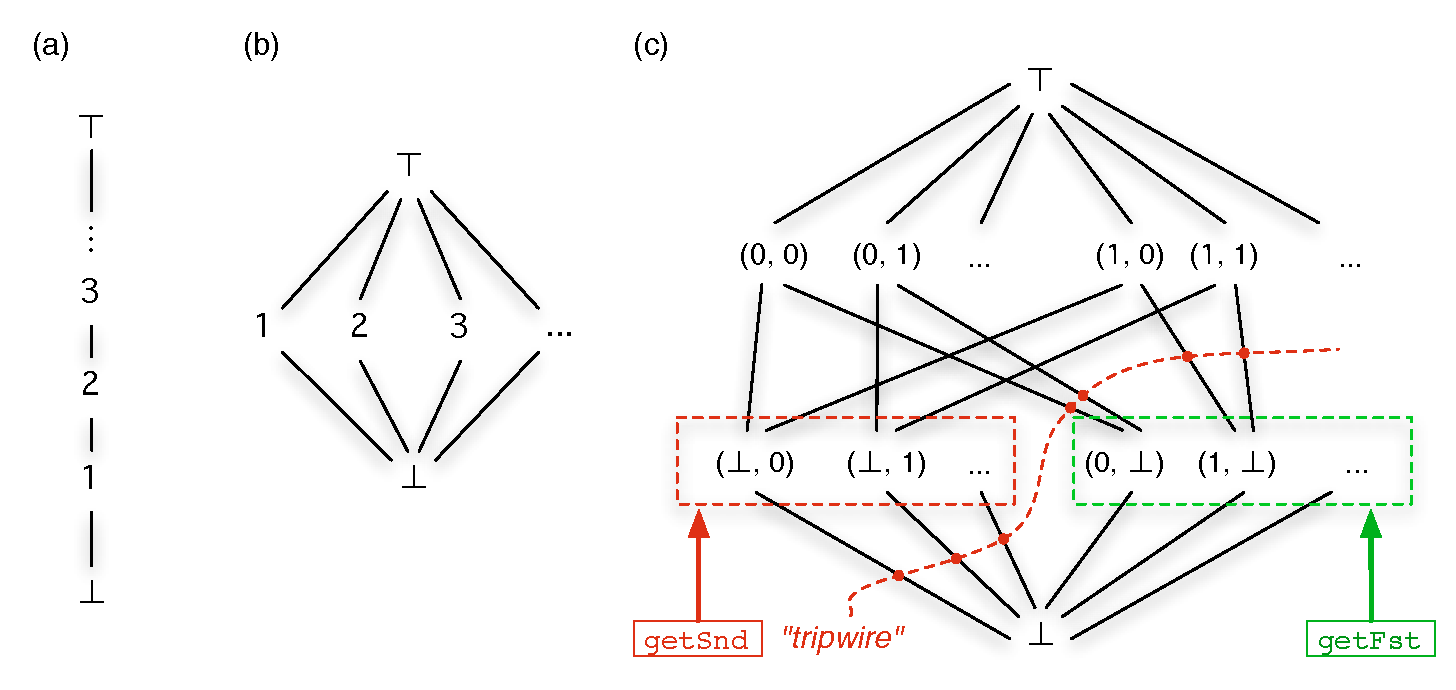
\includegraphics[width=3.3in]{figures/ExampleLattices3.pdf} 
  \caption{Example LVar lattices: (a)
    positive integers ordered by $\leq$; (b) IVar
    containing a positive integer; (c) pair of natural-number-valued IVars, 
    annotated with example threshold
    sets that would correspond to a blocking read of the first or
    second element of the pair.
    Any state transition crossing the
    ``tripwire'' for \termfont{getSnd} causes it to unblock
    and return a result.}

  \label{f:lattice-examples}
\end{figure}

While the LVar interface just described is deterministic, it is only useful for
synchronization, not for communicating data: we must specify in advance the
single answer we expect to be returned from the call to $\GET$.  In general,
though, threshold sets do not have to be singleton sets.  For example, consider
an LVar $\mathit{lv}$ whose states form a lattice of \emph{pairs} of
natural-number-valued IVars; that is, $\mathit{lv}$ is a pair $(m, n)$, where
$m$ and $n$ both start as $\bot$ and may each be updated once with a non-$\bot$
value, which must be some natural number.
This lattice is shown in Figure~\ref{f:lattice-examples}(c).

We can then define $\GETFST$ and
$\GETSND$ operations for reading from the first and second entries of
$\mathit{lv}$:
\begin{align*}
\getfstexp{p} & \defeq \getexp{p}{\stateset{(m, \bot) \setsep m \in
    \mathbb{N}}} \\
\getsndexp{p} & \defeq \getexp{p}{\stateset{(\bot, n) \setsep n \in
    \mathbb{N}}}
\end{align*}
This allows us to write programs like the following:
\begin{equation}
\begin{split}
& \LETPAR ~\_ = \putexp{\mathit{lv}}{(\bot, 4)} \\
&  \letparspace ~\_ = \putexp{\mathit{lv}}{(3, \bot)} \\
&  \letparspace ~x = \getsndexp{\mathit{lv}} \\
&  \letspace \IN~x
%% \LETPAR ~\_ = \putexp{\mathit{lv}}{(\bot, 4)};~
%%  ~\_ = \putexp{\mathit{lv}}{(3, \bot)};~
%%  ~x = \getsndexp{\mathit{lv}} ~~ \IN~x
\end{split}
\label{e:lvar-example-4}
\end{equation}
In the call $\getsndexp{\mathit{lv}}$, the threshold set is
 $\setof{(\bot, 0), (\bot, 1),  \dots}$, an infinite set.  There
is no risk of nondeterminism because the elements of the threshold set
are \emph{pairwise incompatible} with respect to $\mathit{lv}$'s lattice:
informally, since the second entry of $\mathit{lv}$ can only be
written once, no more than one state from the set $\setof{(\bot, 0),
  (\bot, 1),  \dots}$ can ever be reached.  (We formalize
this incompatibility requirement in
Section~\ref{subsection:newputget}.)  

%% Therefore, for any given
%% program, $\GET$ will behave deterministically regardless of the size
%% of the threshold set, so long as the elements of the threshold set are
%% incompatible.\if 0\footnote{With one exception: $\GET$ can behave
%%   nondeterministically in the case of a program that is
%%   going to raise an error anyway; see Section~\ref{subsection:newputget}.}\fi

In the case of \ref{e:lvar-example-4}, $\getsndexp{\mathit{lv}}$ may unblock and
return $(\bot, 4)$ any time after the second entry of $\mathit{lv}$ has been
written, regardless of whether the first entry has been written yet.  It is
therefore possible to use LVars to safely read parts of an incomplete data
structure---say, an object that is in the process of being initialized by a
constructor.

\paragraph{The model versus reality}

The use of explicit threshold sets in the above LVars model should be understood
as a mathematical modeling technique, \emph{not} an implementation approach or
practical API.  Our library (discussed in Section~\ref{section:implementation})
provides an unsafe \texttt{getLV} operation to the authors of LVar data structure
libraries, who can then make operations like $\GETFST$ and $\GETSND$ available as a safe
interface for application writers, implicitly baking in the particular threshold sets that make
sense for a given data structure without ever explicitly constructing them.

To put it another way, operations on a data structure exposed as an LVar must have
the \emph{semantic effect} of a least upper bound for writes or a threshold for
reads, but none of this need be visible to clients (or even written explicitly
in the code).  Any data structure API that provides such a semantics is
guaranteed to provide deterministic concurrent communication.



\section{LVish, informally}\label{s:quasi-informal}

\ifdefined\DISSERTATION
While LVars offer a deterministic programming model that allows
communication through a wide variety of data structures, they are not
powerful enough to express common algorithmic patterns, like fixpoint
computations, that require both positive and negative queries.
\fi
In
this section, \either{I}{we} explain our extensions to the LVars model at a high
level; Section~\ref{s:quasi-formal} then formalizes them.

\subsection{Asynchrony through event handlers}

Our first extension to LVars is the ability to do asynchronous,
event-driven programming through event handlers.  An \emph{event} for
an LVar can be represented by a lattice element; the event
\emph{occurs} when the LVar's current value reaches a point at or
above that lattice element.  An \emph{event handler} ties together an
LVar with a callback function that is asynchronously invoked whenever
some events of interest occur.

To illustrate how event handlers work, consider again the lattice of
Figure~\ref{f:lvars-example-lattices}(a) from Chapter~\ref{ch:lvars}.
Suppose that $\mathit{lv}$ is an LVar whose states correspond to this
lattice.  The expression

\singlespacing
\begin{equation}
  \ADDHANDLER~\mathit{lv}~\{ 1, 3, 5, \dots \}~(\lam{x}{\putexp{\mathit{lv}}{x+1}})
\label{e:lvish-example-1}
\end{equation}
\doublespacing

registers a handler for $\mathit{lv}$ that executes the callback
function $\lam{x}{\putexp{\mathit{lv}}{x+1}}$ for each odd number that
$\mathit{lv}$ is at or above.  When \eref{e:lvish-example-1} is
finished evaluating, $\mathit{lv}$ will contain the smallest even
number that is at or above what its original value was.  For instance,
if $\mathit{lv}$ originally contains $4$, the callback function will
be invoked twice, once with $1$ as its argument and once with $3$.
These calls will respectively write $1+1 = 2$ and $3+1 = 4$ into
$\mathit{lv}$; since both writes are $\leq 4$, $\mathit{lv}$ will
remain $4$.  On the other hand, if $\mathit{lv}$ originally contains
$5$, then the callback will run three times, with $1$, $3$, and $5$ as
its respective arguments, and with the latter of these calls writing
$5+1 = 6$ into $\mathit{lv}$, leaving $\mathit{lv}$ as $6$.

In general, the second argument to @addHandler@, which \either{I}{we} call an
\emph{event set}, is an arbitrary subset $Q$ of the LVar's lattice,
specifying which events should be handled.\footnote{Like threshold
  sets, these event sets are a mathematical modeling tool only; they
  have no explicit existence in the LVish library implementation.}
Event handlers in the LVish model are somewhat unusual in that they
invoke their callback for \emph{all} events in their event set $Q$
that have taken place (\ie, all values in $Q$ less than or equal to
the current LVar value), even if those events occurred prior to the
handler being registered.  To see why this semantics is necessary,
consider the following, more subtle example (written in a hypothetical
language with a semantics similar to that of $\lambdaLVar$, but with
the addition of @addHandler@):

\singlespacing
\begin{equation}
\begin{split}
& \LETPAR ~\_ = \putexp{\mathit{lv}}{0} \\
&  \letparspace ~\_ = \putexp{\mathit{lv}}{1} \\
&  \letparspace ~\_ = \ADDHANDLER~\mathit{lv}~\{ 0, 1 \}~
     (\lam{x}{\termfont{if}~x=0~\termfont{then}~\putexp{\mathit{lv}}{2}}) \\
&  \letspace \IN~ \getexp{\mathit{lv}}{\setof{2}}
\end{split}
\label{e:lvish-example-2}
\end{equation}
\doublespacing

Can~\eref{e:lvish-example-2} ever block?  If a callback only executed
for events that arrived after its handler was registered, or only for
the largest event in its event set that had occurred, then the
example would be nondeterministic: it would block, or not, depending
on how the handler registration was interleaved with the
\termfont{put}s.  By instead executing a handler's callback once for
\emph{each and every} element in its event set below or at the LVar's
value, we guarantee quasi-determinism---and, for
\eref{e:lvish-example-2}, guarantee the result of $2$.

The power of event handlers is most evident for lattices that model
collections, such as sets.  For example, if we are working with
lattices of sets of natural numbers, ordered by subset inclusion, then
we can write the following function:
\[
\termfont{forEach} = \lam{\mathit{lv}}{
  \lam{f}{
    \ADDHANDLER~\mathit{lv}~\{ \{0\}, \{1\}, \{2\}, \dots \}~f
  }}
\]
Unlike the usual @forEach@ function found in functional programming
languages, this function sets up a \emph{permanent}, asynchronous flow
of data from $\mathit{lv}$ into the callback $f$.  Functions like
@forEach@ can be used to set up complex, cyclic data-flow networks, as
we will see in Chapter~\ref{ch:lvish}.

In writing @forEach@, we consider only the singleton sets to be events
of interest, which means that if the value of $\mathit{lv}$ is some
set like $\setof{2, 3, 5}$ then $f$ will be executed once for each
singleton subset ($\setof{2}$, $\setof{3}$, $\setof{5}$)---that is,
once for each element.  In Chapter~\ref{ch:lvish}, we will see that
this kind of event set can be specified in a lattice-generic way, and
that it corresponds closely to our implementation strategy.

\subsection{Quiescence through handler pools}\label{subsection:quasi-quiescence}

Because event handlers are asynchronous, we need a separate mechanism
to determine when they have reached a \emph{quiescent} state, \ie,
when all callbacks for the events that have occurred have finished
running.  As we saw in the introduction to this chapter, detecting
quiescence is crucial for implementing fixpoint computations.  To
build flexible data-flow networks, it is also helpful to be able to
detect quiescence of multiple handlers simultaneously.  Thus, our
design includes \emph{handler pools}, which are groups of event
handlers whose collective quiescence can be tested.

The simplest way to program with handler pools is to use a pattern
like the following:

\singlespacing
\[
\begin{array}[t]{l}
\termfont{let}~\mathit{h}~=~\NEWPOOL \\
\letspace \termfont{in}
  \begin{array}[t]{l}
    \ADDHANDLERINPOOL~h~\mathit{lv}~Q~f; \\
    \QUIESCE~h
  \end{array}
\end{array}
\]
\doublespacing

where $\mathit{lv}$ is an LVar, $Q$ is an event set, and $f$ is a
callback.  Handler pools are created with the @newPool@ function, and
handlers are registered with @addHandlerInPool@, a variant of
@addHandler@ that takes a handler pool as an additional argument.
Finally, @quiesce@ takes a handler pool as its argument and blocks
until all of the handlers in the pool have reached a quiescent state.

Of course, whether or not a handler is quiescent is a non-monotonic
property: we can move in and out of quiescence as more writes to an
LVar occur, and even if all states at or below the current state have
been handled, there is no way to know that more writes will not arrive
to move the LVar's state upwards in the lattice and trigger more
callbacks.  Early quiescence no risk to quasi-determinism, however,
because @quiesce@ does not yield any information about \emph{which}
events have been handled---any such questions must be asked through
LVar functions like @get@.  In practice, @quiesce@ is almost always
used together with freezing, which \either{I}{we} explain next.

\subsection{Freezing and the ``freeze-after'' pattern}\label{subsection:quasi-freeze-after}

Our final addition to the LVar model is the ability to \emph{freeze}
an LVar, which forbids further changes to it, but in return allows its
exact value to be read.  We expose freezing through the function
@freeze@, which takes an LVar as its sole argument, and returns the
exact value of the LVar as its result.  Any writes that would change
the value of a frozen LVar instead raise an exception, and it is the
potential for races between such writes and @freeze@ that makes the
LVish model quasi-deterministic, rather than fully deterministic.

Putting all the above pieces together, we arrive at a particularly
common pattern of programming in the LVish model:

\singlespacing
\[
\begin{array}[t]{l}
  \termfont{freezeAfter} = \lam{\mathit{lv}}{\lam{Q}{\lam{f}{}}}
  \begin{array}[t]{l}
    \termfont{let}~\mathit{h}~=~\NEWPOOL \\
    \termfont{in}
      \begin{array}[t]{l}  
        \ADDHANDLERINPOOL~h~\mathit{lv}~Q~f;
\\
        \QUIESCE~h;
\\
        \FREEZE~\mathit{lv}
      \end{array}
  \end{array}
\end{array}
\]
\doublespacing

In this pattern, an event handler is registered for an LVar,
subsequently quiesced, and then the LVar is frozen and its exact value
is returned.

\subsection{A parallel graph traversal using handlers, quiescence, and freezing}\label{subsection:quasi-parallel-graph-traversal}

We can use the new features in LVish to write a parallel graph
traversal in the following simple fashion:

\singlespacing
\lstinputlisting{chapter3/code/bfs_new.hs}
\doublespacing

This code, written using the LVish Haskell library (which \either{I}{we} will go on
to describe in Chapter~\ref{ch:lvish}), discovers (in parallel) the
set of nodes in a graph @g@ reachable from a given node @startV@, and
is guaranteed to produce a deterministic result.\footnote{In the LVish
  library, the \lstinline|Par| type constructor is the monad in which
  LVar computations run; see Chapter~\ref{ch:lvish} for details.}  It
works by creating a fresh @Set@ LVar (corresponding to a lattice whose
elements are sets, with set union as lub), and seeding it with the
starting node.

The @freezeSetAfter@ function implements a set-specific variant of the
freeze-after pattern I described above.  It combines freezing and
event handlers: first, it registers the callback @handle@ as a handler
for the @seen@ set, which will asynchronously put the neighbors of
each visited node into the set, possibly triggering further callbacks,
recursively.  Second, when no further callbacks are ready to
run---\ie, when the @seen@ set has reached a
fixpoint---@freezeSetAfter@ will freeze the set and return its exact
value.


\section{LVish, formally}\label{s:quasi-formal}

In this section, \either{I}{we} present $\lambdaLVish$, a core calculus for the
LVish programming model. $\lambdaLVish$ is a quasi-deterministic,
parallel, call-by-value $\lambda$-calculus extended with a store
containing LVars.  It extends the original $\lambdaLVar$ language of
\either{Chapter}{Section}~\ref{ch:lvars} to support the new features in the LVish model
that \either{I}{we} described in Section~\ref{s:quasi-informal}. Rather than
modeling the full ensemble of event handlers, handler pools,
quiescence, and freezing as separate primitives, \either{I}{we} instead formalize
the ``freeze-after'' pattern---which combined them---directly as a
primitive.  This simplifies the calculus while still capturing the
essence of the programming model.  \either{I}{We} also generalize the @put@
operation to allow arbitrary \emph{update operations} (previously
described in
Section~\either{\ref{subsection:lvars-generalizing-from-least-upper-bound-writes}}{\ref{s:lvars-generalizing}}),
which are inflationary and commutative, but do not necessarily compute
a lub.

\subsection{Lattices}

Just as with $\lambdaLVar$, the application-specific lattice is given
as a 4-tuple $(D, \userleq, \bot, \top)$ where $D$ is a set,
$\userleq$ is a partial order on the elements of $D$, $\bot$ is the
least element of $D$ according to $\userleq$ and $\top$ is the
greatest.  The $\bot$ element represents the initial ``empty'' state
of every LVar, while $\top$ represents the ``error'' state that would
result from conflicting updates to an LVar.  The partial order
$\userleq$ represents the order in which an LVar may take on states.
It induces a binary lub operation $\userlub{}{}$ on the elements of
$D$.  Every two elements of $D$ must have a lub in $D$.  Formally,
this makes $(D, \userleq, \bot, \top)$ a \emph{bounded
  join-semilattice} with a designated greatest element $\top$; \either{I}{we}
continue to use ``lattice'' as shorthand, and \either{I}{we} use $D$ as a shorthand
for the entire 4-tuple $(D, \userleq, \bot, \top)$ when its meaning is
clear from the context. \lk{Hm, do I actually do that?}

\subsection{Freezing}

To model freezing, we need to generalize the notion of the state of an
LVar to include information about whether it is ``frozen'' or not.
Thus, in $\lambdaLVish$ an LVar's \emph{state} is a pair
$\state{d}{\status}$, where $d$ is an element of the
application-specific set $D$ and $\status$ is a ``status bit'' of
either $\frozentrue$ or $\frozenfalse$.  A state where $\status$ is
$\frozenfalse$ is ``unfrozen'', and one where $\status$ is
$\frozentrue$ is ``frozen''.

\either{I}{We} define an ordering $\leqp$ on LVar states $\state{d}{\status}$ in
terms of the application-specific ordering $\userleq$ on elements of
$D$.  Every element of $D$ is ``freezable'' except $\top$.
Informally:
\begin{itemize}
\item Two unfrozen states are ordered according to the
  application-specific $\userleq$; that is, $\state{d}{\frozenfalse}
  \leqp \state{d'}{\frozenfalse}$ exactly when $d \userleq d'$.
\item Two frozen states do not have an order, unless they are equal:
  $\state{d}{\frozentrue} \leqp \state{d'}{\frozentrue}$ exactly when
  $d = d'$.
\item An unfrozen state $\state{d}{\frozenfalse}$ is less than or
  equal to a frozen state $\state{d'}{\frozentrue}$ exactly when $d
  \userleq d'$.
\item The only situation in which a frozen state is less than an
  unfrozen state is if the unfrozen state is $\top$; that is,
  $\state{d}{\frozentrue} \leqp \state{d'}{\frozenfalse}$ exactly when
  $d' = \top$.
\end{itemize}
Adding status bits to each element (except $\top$) of the lattice $(D,
\userleq, \bot, \top)$ results in a new lattice $(D_p, \leqp, \botp,
\topp)$.  (The $p$ stands for pair, since elements of this new lattice
are pairs $\state{d}{\status}$.) \either{I}{We} write $\lubp{}{}$ for the lub
operation that $\leqp$ induces.
Definitions~\ref{def:lattice-with-status-bits} and \ref{def:lubp} and
Lemmas~\ref{lem:partition-of-Dp} and~\ref{lem:lattice-structure}
formalize this notion.
\ifdefined\JOURNAL
As before, we only give the statements of the lemmas here; the proofs
appear in~\cite{lvars-dissertation}.
\fi

\DefLatticeWithStatusBits

\LemPartitionOfDp
\ifdefined\DISSERTATION
\begin{proof}
  Immediate from Definition~\ref{def:lattice-with-status-bits}.
\end{proof}
\fi

\DefLubP

Lemma~\ref{lem:lattice-structure} says that if $(D, \leq, \bot, \top)$
is a lattice, then $(D_p, \leqp, \botp, \topp)$ is as well:

\LemLatticeStructure
\ifdefined\DISSERTATION
\begin{proof}
See Section~\ref{section:lattice-structure-proof}.
\end{proof}
\fi

\subsection{Update operations}\label{subsection:quasi-update-operations}

$\lambdaLVish$ generalizes the @put@ operation of $\lambdaLVar$ to a
family of operations $\PUTi$, in order to allow the generalized update
operations of
Section~\either{\ref{subsection:lvars-generalizing-from-least-upper-bound-writes}}{\ref{s:lvars-generalizing}}
that are commutative and inflationary, but do not necessarily compute
a lub.  To make this possible we parameterize $\lambdaLVish$ not only
by the lattice $(D, \userleq, \bot, \top)$, but also by a set $U$ of
\emph{update operations}, as discussed previously in
Section~\either{\ref{subsection:lvars-generalizing-from-least-upper-bound-writes}}{\ref{s:lvars-generalizing}}:

\DefSetOfUpdateOperations

The first of the conditions in
Definition~\ref{def:set-of-update-operations} says that each update
operation is inflationary with respect to $\userleq$, and the second
condition says that update operations commute with each other.  Every
set of update operations always implicitly contains the identity
function.

If we want to encode the original lub semantics of @put@ using
$\PUTi$, we can do so by instantiating $U$ such that there is one
$u_i$ for each element $d_i$ of the lattice $D$, and defining $u_i(d)$
to be $\userlub{d}{d_i}$.  On the other hand, if $D$ is a lattice of
natural numbers and we want increment-only counters, we can
instantiate $U$ to be a singleton set $\setof{ u }$ where $u(d) = d +
1$.  (As described in
Section~\either{\ref{subsection:lvars-generalizing-from-least-upper-bound-writes}}{\ref{s:lvars-generalizing}},
we could also have a set of update operations $\{ u_{(+1)}, u_{(+2)},
\dots \}$, where $u_{(+1)}(d)$ increments $d$'s contents by one,
$u_{(+2)}(d)$ increments by two, and so on.) Update operations are
therefore general enough to express lub writes as well as
non-idempotent increments.  (When a write is specifically a lub write,
\either{I}{we} will continue to use the notation @put@, without the subscript.)

In $\lambdaLVish$, the @put@ operation took two arguments, a location
$l$ and a lattice element $d$.  The $\PUTi$ operations take a location
$l$ as their only argument, and $\putiexp{l}$ performs the update
operation $u_i(l)$ on the contents of $l$.

More specifically, since $l$ points to a state $\state{d}{\status}$
instead of an element $d$, $\putiexp{l}$ must perform $u_{p_i}$, a
lifted version of $u_i$ that applies to states.  Given $U$, we define
the set $U_p$ of lifted operations as follows:

\DefSetOfStateUpdateOperations

Because every set $U$ of update operations implicitly contains the
identity function, the same is true for the set $U_p$ of state update
operations.  Furthermore, it is easy to show that state update
operations commute, just as update operations do; that is, $\forall d,
i, j.  \;\; u_{p_i}(u_{p_j}(p)) = u_{p_j}(u_{p_i}(p))$. \lk{I've done
  the proof of this, but I'm not including it here because it seems
  pretty obvious from the definition...if anyone wants me to actually
  include it, then I will.}

\subsection{Stores}

During the evaluation of $\lambdaLVish$ programs, a \emph{store} $S$
keeps track of the states of LVars.  Each LVar is represented by a
binding from a location $l$, drawn from a set $\Loc$, to its state,
which is some pair $\state{d}{\status}$ from the set $D_p$.  The way
that stores are handled in $\lambdaLVish$ is very similar to how they
are handled in $\lambdaLVar$, except that store bindings now point to
states $\state{d}{\status}$, that is, elements of $D_p$, instead of
merely to $d$, that is, elements of $D$.

\DefStore

\either{I}{We} use the notation $\extS{S}{l}{d}{\status}$ to denote extending $S$
with a binding from $l$ to $\state{d}{\status}$.  If $l \in \dom{S}$,
then $\extS{S}{l}{d}{\status}$ denotes an update to the existing
binding for $l$, rather than an extension.  Another way to denote a
store is by explicitly writing out all its bindings, using the
notation $\store{\storebinding{l_1}{d_1}{\status_1},
  \storebinding{l_2}{d_2}{\status_2}, \dots}$.

We can lift the $\leqp$ and $\lubp{}{}$ operations defined on elements
of $D_p$ to the level of stores:

\DefLeqStore

\DefLubStore

If, for example,
\[ \lubp{\state{d_1}{\status_1}}{\state{d_2}{\status_2}} = \topp, \]
then
\[ \lubstore{\store{\storebinding{l}{d_1}{\status_1}}}{\store{\storebinding{l}{d_2}{\status_2}}} =
\topS. \]

Just as a store containing a binding $\storebindingRaw{l}{\top}$ can
never arise during the execution of a $\lambdaLVar$ program, a store
containing a binding $\storebinding{l}{\top}{\status}$ can never arise
during the execution of a $\lambdaLVish$ program. An attempted write
that would take the value of $l$ to
$\state{\top}{\frozenfalse}$---that is, $\topp$---will raise an error,
and there is no $\state{\top}{\frozentrue}$ element of $D_p$.

\subsection{$\lambdaLVish$: syntax and semantics}

The syntax of $\lambdaLVish$ appears in
Figure~\ref{f:lambdaLVish-syntax}, and
Figures~\ref{f:lambdaLVish-reduction-semantics}
and~\ref{f:lambdaLVish-context-semantics} together give the
operational semantics.  As with $\lambdaLVar$ in
\either{Chapter}{Section}~\ref{ch:lvars}, both the syntax and semantics are
parameterized by the lattice $(D, \userleq, \bot, \top)$, and the
operational semantics is split into two parts, a \emph{reduction
  semantics}, shown in
Figure~\ref{f:lvars-lambdaLVar-reduction-semantics}, and a
\emph{context semantics}, shown in
Figure~\ref{f:lvars-lambdaLVar-context-semantics}.  The reduction
semantics is also parameterized by the set $U$ of update operations.

\FigLambdaLVishGrammar

\FigLambdaLVishReductionSemantics

\FigLambdaLVishContextSemantics

The $\lambdaLVish$ grammar has most of the expression forms of
$\lambdaLVar$: variables, values, application expressions, @get@
expressions, and @new@.  Instead of @put@ expressions, it has $\PUTi$
expressions, which are the interface to the specified set of update
operations.  $\lambdaLVish$ also adds two new language forms, the
@freeze@ expression and the $\FAW$ expression, which \either{I}{we} discuss in more
detail below.

Values in $\lambdaLVish$ include all those from $\lambdaLVar$---the
unit value $\unit$, lattice elements $d$, locations $l$, threshold
sets $P$, and $\lambda$ expressions---as well as states $p$, which are
pairs $\state{d}{\status}$, and event sets $Q$.  Instead of $T$, \either{I}{we} now
use the metavariable $P$ for threshold sets, in keeping with the fact
that in $\lambdaLVish$, members of threshold sets are states $p$.

As before, configurations $\config{S}{e}$ are made up of a store and
an expression; the \emph{error configuration}, written $\error$, is a
unique element added to the set of configurations, but
$\config{\topS}{e}$ is equal to $\error$ for all expressions $e$; and
the metavariable $\conf$ ranges over configurations.  Both the
reduction relation $\parstepsto$ and the context relation
$\ctxstepsto$ are defined on configurations.

As with $\lambdaLVar$, the $\lambdaLVish$ context relation
$\ctxstepsto$ has only one rule, {\sc E-Eval-Ctxt}, which allows us to
apply reductions within a context. The rule itself is identical to the
corresponding rule in $\lambdaLVar$, although the set of evaluation
contexts that the metavariable $E$ ranges over is different.

\subsection{Semantics of \il{new}, $\PUTi$, and \il{get}}\label{subsection:quasi-semantics-of-new-put-and-get}

Because of the addition of status bits to the semantics, the {\sc
  E-New} and {\sc E-Get} rules have changed slightly from their
counterparts in $\lambdaLVar$:

\begin{itemize}
\item @new@ (implemented by the {\sc E-New} rule) extends the store
  with a binding for a new LVar whose initial state is $(\bot,
  \frozenfalse)$, and returns the location $l$ of that LVar (\ie, a
  pointer to the LVar).
\item @get@ (implemented by the {\sc E-Get} rule) performs a blocking
  threshold read.  It takes a pointer to an LVar and a \emph{threshold
    set} $P$, which is a non-empty set of LVar states that must be
  \emph{pairwise incompatible}, expressed by the premise $\incomp{P}$.
  A threshold set $P$ is pairwise incompatible iff the lub of any two
  distinct elements in $P$ is $\topp$.  If the LVar's state $p_1$ in
  the lattice is \emph{at or above} some $p_2 \in P$, the @get@
  operation unblocks and returns $p_2$.  Note that $p_2$ is a unique
  element of $P$, for if there is another $p'_2 \neq p_2$ in the
  threshold set such that $p'_2 \leqp p_1$, it would follow that
  $\lubp{p_2}{p'_2} = p_1 \neq \topp$, which contradicts the
  requirement that $P$ be pairwise incompatible.
\end{itemize}

$\lambdaLVish$'s counterpart to the @put@ operation is the $\PUTi$
operation, which is actually a set of operations that provide access
to the provided update operations $u_i$.  For each $u_i$ update
operation, $\PUTi$ (implemented by the {\sc E-Put} rule) takes a
pointer to an LVar and updates the LVar's state to result of calling
$u_{p_i}$ on the LVar's current state, potentially pushing the state
of the LVar upward in the lattice.  The {\sc E-Put-Err} rule applies
when a $\PUTi$ operation would take the state of an LVar to $\topp$;
in that case, the semantics steps to $\error$.

\subsection{Freezing and the $\FAW$ primitive}\label{subsection:quasi-freezing}

The {\sc E-Freeze-Init}, {\sc E-Spawn-Handler}, {\sc E-Freeze-Final},
and {\sc E-Freeze-Simple} rules are all new additions to
$\lambdaLVish$.  The {\sc E-Freeze-Simple} rule gives the semantics
for the @freeze@ expression, which takes an LVar as argument and
immediately freezes and returns its contents.

More interesting is the $\FAW$ primitive, which models the
``freeze-after'' pattern \either{I}{we} described in
Section~\ref{subsection:quasi-freeze-after}.  The expression
\[ \freezeafter{e_{\rm lv}}{e_{\rm events}}{e_{\rm cb}} \]
has the following semantics:
\begin{itemize}
\item It attaches the callback $e_{\rm cb}$ to the LVar $e_{\rm lv}$.
  The expression $e_{\rm events}$ must evaluate to a event set $Q$;
  the callback will be executed, once, for each lattice element in $Q$
  that the LVar's state reaches or surpasses.  The callback $e_{\rm
    cb}$ is a function that takes a lattice element as its argument.
  Its return value is ignored, so it runs solely for effect.  For
  instance, a callback might itself do a $\PUTi$ to the LVar to which
  it is attached, triggering yet more callbacks.
\item If the handler reaches a quiescent state, the LVar $e_{\rm lv}$
  is frozen, and its \emph{exact} state is returned (rather than an
  underapproximation of the state, as with @get@).
\end{itemize}
To keep track of the running callbacks, $\lambdaLVish$ includes an
auxiliary form,
\[
\freezeafterfull{l}{Q}{\lam{x}{e_0}}{\setof{e, \dots}}{H}
\]
where:
\begin{itemize}
\item The value $l$ is the LVar being handled/frozen;
\item The set $Q$ (a subset of the lattice $D$) is the event set;
\item The value $\lam{x}{e_0}$ is the callback function;
\item The set of expressions $\setof{e, \dots}$ are the running
  callbacks; and
\item The set $H$ (a subset of the lattice $D$) represents those
  values in $Q$ for which callbacks have already been launched.
\end{itemize}
Due to $\lambdaLVish$'s use of evaluation contexts, any running
callback can execute at any time, as if each is running in its own
thread.

The rule {\sc E-Spawn-Handler} launches a new callback thread any time
the LVar's current value is at or above some element in $Q$ that has
not already been handled.  This step can be taken nondeterministically
at any time after the relevant $\PUTi$ has been performed.

The rule {\sc E-Freeze-Final} detects quiescence by checking that two
properties hold.  First, every event of interest (lattice element in
$Q$) that has occurred (is bounded by the current LVar state) must be
handled (be in $H$).  Second, all existing callback threads must have
terminated with a value.  In other words, every enabled callback has
completed.  When such a quiescent state is detected, {\sc
  E-Freeze-Final} freezes the LVar's state.  Like {\sc
  E-Spawn-Handler}, the rule can fire at any time,
nondeterministically, that the handler appears quiescent---a transient
property!  But after being frozen, any further $\PUTi$ updates that
would have enabled additional callbacks will instead fault, causing
the program to step to $\error$.

Therefore, freezing is a way of ``betting'' that once a collection of
callbacks have completed, no further updates that change the LVar's
value will occur.  For a given run of a program, either all updates to
an LVar arrive before it has been frozen, in which case the value
returned by $\FAW$ is the lub of those values, or some update arrives
after the LVar has been frozen, in which case the program will fault.
And thus we have arrived at \emph{quasi-determinism}: a program will
always either evaluate to the same answer or it will fault.

To ensure that we will win our bet, we need to guarantee that
quiescence is a \emph{permanent} state, rather than a transient
one---that is, we need to perform all updates either prior to $\FAW$,
or by the callback function within it (as will be the case for
fixpoint computations).  In practice, freezing is usually the very
last step of an algorithm, permitting its result to be extracted. As
we will see in
Section~\ref{subsection:lvish-regaining-full-determinism-with-runparthenfreeze},
our LVish library provides a special @runParThenFreeze@ function that
does so, and thereby guarantees full determinism.


\section{Quasi-Determinism for LVish}\label{section:proof}

Our proof of quasi-determinism for LVish formalizes the claim we make
in Section~\ref{section:intro}: that, for a given program, although
some executions may raise exceptions, all executions that produce a
final result will produce the same final result.

In this section, we give the statements of the main
quasi-determinism theorem and the two most important supporting
lemmas.  The statements of the remaining lemmas,
and proofs of all our theorems and lemmas,
are included in
\ifx\fulltr\undefined
%%% Text for paper
the companion
technical report \cite{Freeze-TR}.
\else
%%% Text for TR
Appendix~\ref{app:quasi-determinism-for-lvish}.
\fi

\subsection{Quasi-Determinism and Quasi-Confluence}

Our main result, Theorem~\ref{thm:quasi-determinism}, says that if two
executions starting from a configuration $\conf$ terminate in
configurations $\conf'$ and $\conf''$, then $\conf'$ and $\conf''$ are
the same configuration, or one of them is $\error$.

\ThmQuasiDeterminism

\noindent Theorem~\ref{thm:quasi-determinism} follows from a series of
\emph{quasi-confluence} lemmas.  The most important of these,
Strong Local Quasi-Confluence (Lemma~\ref{lem:strong-local-quasi-confluence}), says that if a
configuration steps to two different configurations, then either there
exists a single third configuration to which they both step (in at
most one step), or one of them steps to $\error$.
Additional lemmas generalize Lemma~\ref{lem:strong-local-quasi-confluence}'s result to multiple
steps by induction on the number of steps, eventually building up to Theorem~\ref{thm:quasi-determinism}.

\LemStrongLocalQuasiConfluence

\if 0
\noindent The Strong Quasi-Confluence lemma,
Lemma~\ref{lem:strong-quasi-confluence}, immediately implies
Quasi-Confluence, Lemma~\ref{lem:quasi-confluence}.  Although the
weaker property Quasi-Confluence is all that is necessary to show
Theorem~\ref{thm:quasi-determinism}, Strong Quasi-Confluence is an
interesting result in itself because it bounds the number of steps
that an execution will take to reach $\error$.
\fi

\subsection{Independence}

In order to show
Lemma~\ref{lem:strong-local-quasi-confluence},
%% on which the rest of
%% the quasi-confluence lemmas and ultimately
%% Theorem~\ref{thm:quasi-determinism} depend,
%% we are required to
we need a ``frame property'' for LVish that captures the idea that
independent effects commute with each other.
Lemma~\ref{lem:independence}, the Independence lemma, establishes this
property.  Consider an expression $e$ that runs starting in store $S$
and steps to $e'$, updating the store to $S'$.  The Independence lemma
allows us to make a double-edged guarantee about what will happen if
we run $e$ starting from a larger store $\lubstore{S}{S''}$: first, it
will update the store to $\lubstore{S'}{S''}$; second, it will step to
$e'$ as it did before.\lk{Aaron: Do you think it's fair to claim that
  these respectively boil down to the Safety Monotonicity and Frame
  Property claims from the ``Local Action'' paper?}  Here
$\lubstore{S}{S''}$ is the least upper bound of the original $S$ and
some other store $S''$ that is ``framed on'' to $S$; intuitively,
$S''$ is the store resulting from some other independently-running computation.

\LemIndependence

\noindent Lemma~\ref{lem:independence} requires as a precondition that
the stores $\lubstore{S'}{S''}$ and $S$ are \emph{equal in
  status}---that, for all the locations shared between them, the
status bits of those locations agree.  This assumption rules out
interference from freezing.  Finally, the store $S''$ must be
\emph{non-conflicting} with the original transition from
$\config{S}{e}$ to $\config{S'}{e'}$, meaning that locations in $S''$
cannot share names with locations newly allocated during the
transition; this rules out location name conflicts caused by
allocation.

\DefEqualStatus

\DefNonConflicting










